\chapter{Interactions particule--matière et développement des gerbes}
\label{sec:interactions}

La réponse d'un détecteur calorimétrique repose directement sur les mécanismes d'interaction entre
les particules incidentes et la matière absorbante. Selon leur nature, leur charge et leur énergie,
ces particules déposent leur énergie par ionisation, rayonnement ou interactions nucléaires, donnant
naissance à des cascades secondaires appelées \textbf{gerbes}. La compréhension de ces phénomènes
est essentielle pour interpréter la réponse du SDHCAL et améliorer les performances de
reconstruction étudiées dans ce mémoire.

% ─────────────────────────────────────────────────────────────────────────────
\section{Interaction des particules avec la matière}
\label{sec:interactions-matiere}

\subsection{Interactions des particules chargées}

Dans un milieu, une particule chargée perd principalement de l'énergie par \textbf{ionisation} et
\textbf{excitation} des atomes. La dépendance moyenne du pouvoir d'arrêt suit la loi de
Bethe--Bloch \cite{bichsel1988, pdg2024} :

\begin{equation}
\left\langle -\frac{\mathrm{d}E}{\mathrm{d}x} \right\rangle
= K\,z^{2}\,\frac{Z}{A}\,\frac{1}{\beta^{2}}
\left[
\frac{1}{2}\ln\!\left(
\frac{2 m_{e} c^{2}\,\beta^{2}\gamma^{2}\,T_{\max}}{I^{2}}
\right)
- \beta^{2} - \frac{\delta}{2}
\right],
\label{eq:bethe-bloch}
\end{equation}

où $K = 4\pi N_A r_e^2 m_e c^2$, $z$ est la charge de la particule incidente, $Z/A$ le rapport
charge/masse du milieu, $I$ le potentiel moyen d'excitation, $T_{\max}$ l'énergie maximale
transférable à un électron libre et $\delta$ le terme de correction de densité \cite{pdg2024}.

Cette expression présente un \textit{minimum d'ionisation} pour $\beta\gamma \simeq 3$--$4$
(régime de la particule au minimum d'ionisation, MIP). Dans la gamme d'énergies considérée pour
le SDHCAL (1--130~GeV), l'ionisation domine pour les hadrons et les muons, ce qui justifie l'usage
du MIP comme unité de calibration et motive la lecture multi-seuils pour caractériser la densité
locale de dépôt.

Les autres mécanismes sont secondaires dans ce contexte :

\begin{itemize}
    \item \textbf{Bremsstrahlung} : dominant seulement pour $e^\pm$ au-delà de l'énergie critique
          $E_c \sim 500/Z$~MeV ; négligeable pour hadrons et muons aux énergies visées.
    \item \textbf{Diffusions $e$--$e$} (Møller/Bhabha) et annihilation $e^+$ : effets spécifiques
          aux $e^\pm$, marginaux pour la calorimétrie hadronique étudiée ici.
\end{itemize}

\subsection{Interactions des photons}

Les photons interagissent avec la matière via trois processus principaux, dont l'importance relative
dépend de leur énergie \cite{pdg2024} :

\begin{itemize}
    \item à \textbf{basse énergie} (keV), l'\textit{effet photoélectrique} domine ;
    \item aux \textbf{énergies intermédiaires} (quelques MeV), la \textit{diffusion Compton}
          est prépondérante ;
    \item à \textbf{haute énergie} ($\gg 2 m_e c^2$), la \textit{création de paires}
          $\gamma \to e^+e^-$ devient dominante.
\end{itemize}

Dans un calorimètre comme le SDHCAL, ces mécanismes contribuent essentiellement à la composante
électromagnétique des gerbes, notamment via la désintégration $\pi^0 \to \gamma\gamma$.

\subsection{Interactions des hadrons et des neutrons}

Comme les électrons, les hadrons chargés perdent d'abord de l'énergie par ionisation. Mais, soumis
à l'\textbf{interaction forte}, leurs processus d'interaction sont beaucoup plus complexes.

Lorsqu'un hadron incident interagit avec un noyau, il déclenche une \textbf{spallation nucléaire}
\cite{knoll2010, wigmans2000}. Celle-ci se déroule en deux étapes :

\begin{enumerate}
    \item \textbf{Cascade intranucléaire} : le hadron interagit avec un ou plusieurs nucléons,
          induisant des collisions secondaires. Des hadrons supplémentaires peuvent être créés ;
          certains s'échappent du noyau, d'autres sont réabsorbés.
    \item \textbf{Désexcitation du noyau} : évaporation de protons, neutrons et particules
          $\alpha$, suivie d'émission de $\gamma$. Dans les noyaux lourds, la fission est possible.
\end{enumerate}

Ce processus est hautement stochastique. Une fraction de l'énergie reste \textbf{invisible aux
calorimètres} :

\begin{itemize}
    \item énergie de liaison nucléaire consommée lors de la spallation ;
    \item énergie cinétique de recul du noyau résiduel ;
    \item neutrons secondaires faiblement ou tardivement détectés.
\end{itemize}

Les \textbf{hadrons neutres} (comme le $K^0_L$) n'ionisent pas et ne déposent de l'énergie que via
ces interactions nucléaires, ce qui rend leur point de départ de gerbe plus variable.

Les \textbf{neutrons} constituent un cas particulier selon leur énergie \cite{knoll2010} :

\begin{itemize}
    \item \textbf{Diffusion élastique} ($E < 1$--$10$~MeV) : transfert d'énergie cinétique aux
          noyaux, efficace sur l'hydrogène, mais induisant des signaux retardés ou délocalisés.
    \item \textbf{Diffusion inélastique} ($10$--$100$~MeV) : excitation du noyau suivie
          d'émissions $\gamma$, $p$, $n$, $\alpha$, voire fission.
    \item \textbf{Capture radiative} ($E \approx 0$) : absorption par le noyau, désexcitation
          par $\gamma$ ou $\alpha$.
\end{itemize}

La déposition d'énergie des hadrons dans un calorimètre combine donc des processus d'ionisation,
d'interactions fortes et de cascades nucléaires, avec une forte variabilité et une part d'énergie
non détectée. Ces effets expliquent la complexité de la réponse des calorimètres hadroniques et
les difficultés à atteindre une résolution comparable à celle des calorimètres
électromagnétiques \cite{fabjan2003, wigmans2000}.

% ─────────────────────────────────────────────────────────────────────────────
\section{Gerbes électromagnétiques}
\label{sec:gerbes-em}

Les gerbes électromagnétiques (EM) sont initiées par des électrons, des photons, ou par des
$\pi^0 \to \gamma\gamma$ \cite{heitler1954, rossi1952}. Elles résultent de l'alternance entre
\textit{bremsstrahlung} ($e^\pm \to e^\pm\gamma$) et \textit{création de paires}
($\gamma \to e^+e^-$), jusqu'à ce que l'énergie descende sous l'énergie critique $E_c$, où
l'ionisation devient dominante.

La structure longitudinale et transverse des gerbes est caractérisée par deux grandeurs
fondamentales \cite{pdg2024} :

\begin{itemize}
    \item la \textbf{longueur de radiation} $X_0$, définie comme la distance sur laquelle un
          électron perd en moyenne $1/e$ de son énergie par bremsstrahlung, et qui fixe l'échelle
          longitudinale de développement ;
    \item le \textbf{rayon de Molière} $R_M \approx 21\,\mathrm{MeV}\cdot X_0 / E_c$, qui définit
          l'extension transverse (environ 90\% de l'énergie est contenue dans un cylindre de
          rayon $R_M$).
\end{itemize}

Le profil longitudinal d'énergie déposée peut être décrit par \cite{pdg2024} :

\begin{equation}
\frac{\mathrm{d}E}{\mathrm{d}t} = E_0\,b\,\frac{(bt)^{a-1} e^{-bt}}{\Gamma(a)},
\label{eq:longitudinal-em}
\end{equation}

où $t = x/X_0$ est la profondeur réduite et les paramètres $a$, $b$ dépendent du matériau et de
l'énergie incidente. La position du maximum est donnée par $t_{\max} = (a-1)/b$.

Les gerbes électromagnétiques constituent une référence utile : leur développement est compact,
régulier et bien modélisé, contrairement aux gerbes hadroniques.

% ─────────────────────────────────────────────────────────────────────────────
\section{Gerbes hadroniques}
\label{sec:gerbes-had}

Lorsqu'un hadron de haute énergie pénètre dans un matériau absorbant, il initie une
\textbf{gerbe hadronique} — une cascade complexe de particules secondaires résultant d'interactions
nucléaires successives. Contrairement aux gerbes électromagnétiques, les gerbes hadroniques
présentent d'importantes fluctuations événement par événement dans leur composition, leur extension
spatiale et la fraction d'énergie effectivement détectée \cite{wigmans2000, fabjan2003}.

\subsection{Développement de la cascade}

La gerbe débute par une interaction inélastique du hadron incident avec un noyau du milieu,
produisant pions chargés et neutres, kaons, nucléons secondaires et fragments nucléaires. Les
hadrons secondaires suffisamment énergétiques alimentent la cascade en interagissant à leur tour.

Une caractéristique essentielle est la production de $\pi^0$, qui se désintègrent quasi
instantanément :

\[
\pi^0 \rightarrow \gamma\gamma,
\]

initiant des sous-gerbes électromagnétiques imbriquées. La fraction d'énergie dérivée vers cette
composante EM fluctue fortement d'un événement à l'autre et constitue la principale source de
variabilité de la réponse calorimétrique.

\subsection{Longueur d'interaction}

La grandeur gouvernant le développement longitudinal est la \textbf{longueur d'interaction
nucléaire} \cite{pdg2024} :

\begin{equation}
\lambda_I = \frac{A}{N_A\,\rho\,\sigma_{\mathrm{inel}}},
\label{eq:lambda-i}
\end{equation}

où $A$ est la masse molaire du matériau, $\rho$ sa densité, $N_A$ le nombre d'Avogadro et
$\sigma_{\mathrm{inel}}$ la section efficace inélastique hadron-noyau. Dans les matériaux denses
typiques, $\lambda_I \gg X_0$ : les gerbes hadroniques sont plus profondes et plus diffuses que
les gerbes électromagnétiques, imposant des calorimètres plus épais et moins bien contenus.

\begin{table}[!ht]
    \centering
    \caption{Comparaison des longueurs caractéristiques pour quelques matériaux d'absorbeur
             courants \cite{pdg2024}.}
    \label{tab:longueurs-carac}
    \begin{tabular}{lcccc}
        \hline
        \textbf{Matériau} & $Z$ & $X_0$ (cm) & $\lambda_I$ (cm) & $\lambda_I / X_0$ \\
        \hline
        Fer (Fe)      & 26 & 1.76  & 16.77 & 9.5  \\
        Plomb (Pb)    & 82 & 0.56  & 17.59 & 31.4 \\
        Acier inox    & -- & 1.76  & 16.77 & 9.5  \\
        Tungstène (W) & 74 & 0.35  & 9.95  & 28.4 \\
        \hline
    \end{tabular}
\end{table}

\noindent Le Tableau~\ref{tab:longueurs-carac} illustre le fait que, quelle que soit la densité du
matériau, $\lambda_I$ reste toujours bien supérieure à $X_0$, justifiant la profondeur importante
requise pour les calorimètres hadroniques.

\subsection{Fraction électromagnétique et rapport \texorpdfstring{$h/e$}{h/e}}

La fraction d'énergie transférée à la composante EM via la production de $\pi^0$ est appelée
\textbf{fraction électromagnétique} :

\[
f_{\mathrm{em}} = \frac{E_{\mathrm{EM}}}{E_{\mathrm{tot}}}.
\]

En moyenne, $\langle f_{\mathrm{em}} \rangle$ croît avec l'énergie incidente selon une loi
approximative \cite{wigmans2000} :

\begin{equation}
\langle f_{\mathrm{em}} \rangle \approx 1 - \left(\frac{E}{E_0}\right)^{m-1},
\label{eq:fem}
\end{equation}

avec $E_0$ et $m$ des paramètres dépendant du matériau et de l'espèce hadronique. Toutefois,
$f_{\mathrm{em}}$ fluctue fortement d'un événement à l'autre, même à énergie fixée.

La réponse moyenne d'un calorimètre à une gerbe hadronique s'écrit \cite{wigmans2000} :

\begin{equation}
\langle E_{\pi}\rangle = \left[f_{\mathrm{em}} + (1 - f_{\mathrm{em}})\,\frac{h}{e}\right] E,
\label{eq:he}
\end{equation}

où $e$ et $h$ désignent respectivement les réponses électromagnétique et hadronique du détecteur.
Un calorimètre est dit \textbf{compensant} lorsque $h/e = 1$, ce qui minimise les effets des
fluctuations de $f_{\mathrm{em}}$ sur la résolution. Hors compensation, ces fluctuations constituent
la contribution dominante à la non-linéarité et à la dégradation de la résolution énergétique.

\subsection{Énergie invisible}

Une fraction de l'énergie incidente n'est pas convertie en signal mesurable \cite{fabjan2003} :

\begin{itemize}
    \item énergie de liaison nucléaire consommée lors de la spallation ;
    \item énergie cinétique de recul des noyaux résiduels ;
    \item neutrons secondaires peu ou tardivement détectés ;
    \item particules pénétrantes (muons, neutrinos produits dans certaines désintégrations).
\end{itemize}

Cette énergie invisible est intrinsèquement variable d'un événement à l'autre et contribue
directement à la dégradation de la résolution.

\subsection{Effets temporels}

Les cascades hadroniques ont une structure temporelle plus étendue que les gerbes
électromagnétiques. Une partie du signal est déposée rapidement par les particules relativistes,
tandis que d'autres contributions apparaissent plus tardivement via les neutrons ralentis puis
capturés (temps caractéristiques de l'ordre de quelques dizaines de nanosecondes).

La réponse mesurée dépend donc directement de la fenêtre temporelle d'acquisition du détecteur.
Cet aspect est particulièrement pertinent pour le SDHCAL, dont la lecture semi-digitale est
sensible à la chronologie des dépôts, et dont les variables temporelles constituent des
descripteurs potentiellement discriminants pour le PID (voir chapitre~\ref{sec:pid_mlp}).

\subsection{Containment et fluctuations}

Les gerbes hadroniques, en raison de leur grande extension longitudinale et transverse, peuvent
ne pas être totalement contenues dans le volume instrumenté. L'énergie qui s'échappe crée des
\textbf{fuites longitudinales ou latérales} qui s'ajoutent aux autres sources de dégradation.

La paramétrisation standard de la résolution énergétique d'un calorimètre hadronique est
\cite{fabjan2003} :

\begin{equation}
\frac{\sigma(E)}{E} = \frac{a}{\sqrt{E/\mathrm{GeV}}} \oplus b \oplus \frac{c}{E/\mathrm{GeV}},
\label{eq:resolution}
\end{equation}

où $a$ est le terme stochastique (dominé par les fluctuations de $f_{\mathrm{em}}$ et les
fluctuations d'échantillonnage), $b$ le terme constant (effets systématiques, non-uniformités,
fuites) et $c$ le terme de bruit électronique. L'amélioration de la résolution passe avant tout
par la maîtrise du terme $a$, c'est-à-dire par la réduction des effets liés aux fluctuations
hadroniques.

\subsection{Profils spatiaux}

Le profil longitudinal d'une gerbe hadronique présente une montée rapide suivie d'une décroissance
lente. Son profil transverse se compose de :

\begin{itemize}
    \item un \textbf{cœur dense}, enrichi en composante électromagnétique ($\pi^0 \to \gamma\gamma$),
          de rayon caractéristique proche de $R_M$ ;
    \item une \textbf{région périphérique diffuse}, dominée par les hadrons secondaires et les
          neutrons, s'étendant jusqu'à plusieurs $\lambda_I$ transversalement.
\end{itemize}

\begin{figure}[!ht]
    \centering
    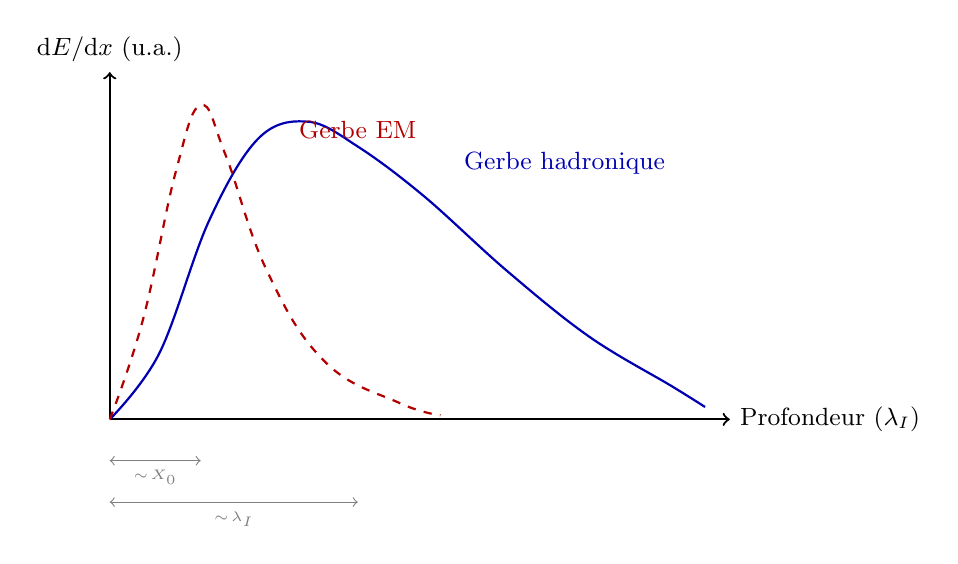
\begin{tikzpicture}[scale=1.05]

        %% ── Axes du profil longitudinal ────────────────────────────────────
        \draw[->, thick] (0,0) -- (7.5,0)
            node[right, font=\small] {Profondeur ($\lambda_I$)};
        \draw[->, thick] (0,0) -- (0,4.2)
            node[above, font=\small] {$\mathrm{d}E/\mathrm{d}x$ (u.a.)};

        %% ── Gerbe hadronique ───────────────────────────────────────────────
        \draw[thick, blue!70!black]
            plot[smooth, tension=0.6] coordinates
            {(0,0)(0.6,0.8)(1.2,2.4)(1.8,3.4)(2.4,3.6)(3.0,3.3)
             (3.8,2.7)(4.8,1.8)(5.8,1.0)(6.8,0.4)(7.2,0.15)};
        \node[blue!70!black, font=\small] at (5.5,3.1)
            {Gerbe hadronique};

        %% ── Gerbe électromagnétique ─────────────────────────────────────
        \draw[thick, red!70!black, dashed]
            plot[smooth, tension=0.7] coordinates
            {(0,0)(0.4,1.2)(0.8,3.0)(1.1,3.8)(1.4,3.2)
             (1.9,1.8)(2.6,0.7)(3.5,0.2)(4.0,0.05)};
        \node[red!70!black, font=\small] at (3.0,3.5)
            {Gerbe EM};

        %% ── Annotations longueurs caractéristiques ───────────────────────
        \draw[<->, gray] (0,-0.5) -- (1.1,-0.5)
            node[midway, below, font=\tiny] {$\sim\! X_0$};
        \draw[<->, gray] (0,-1.0) -- (3.0,-1.0)
            node[midway, below, font=\tiny] {$\sim\! \lambda_I$};

    \end{tikzpicture}

    \vspace{0.8em}

    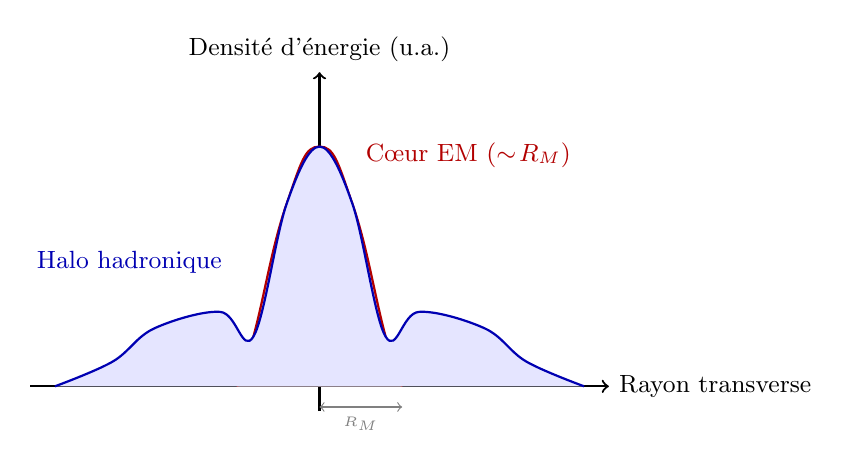
\begin{tikzpicture}[scale=1.05]

        %% ── Vue transversale ───────────────────────────────────────────────
        \draw[->, thick] (-3.5,0) -- (3.5,0)
            node[right, font=\small] {Rayon transverse};
        \draw[->, thick] (0,-0.3) -- (0,3.8)
            node[above, font=\small] {Densité d'énergie (u.a.)};

        %% ── Composante EM (cœur compact) ──────────────────────────────────
        \fill[red!20]
            plot[smooth, tension=0.8] coordinates
            {(-1.0,0)(-0.8,0.6)(-0.4,2.2)(0,2.9)(0.4,2.2)(0.8,0.6)(1.0,0)}
            -- cycle;
        \draw[thick, red!70!black]
            plot[smooth, tension=0.8] coordinates
            {(-1.0,0)(-0.8,0.6)(-0.4,2.2)(0,2.9)(0.4,2.2)(0.8,0.6)(1.0,0)};
        \node[red!70!black, font=\small] at (1.8,2.8)
            {Cœur EM ($\sim\!R_M$)};

        %% ── Halo hadronique ───────────────────────────────────────────────
        \fill[blue!10]
            plot[smooth, tension=0.6] coordinates
            {(-3.2,0)(-2.5,0.3)(-2.0,0.7)(-1.2,0.9)(-0.8,0.6)
             (-0.4,2.2)(0,2.9)(0.4,2.2)(0.8,0.6)(1.2,0.9)
             (2.0,0.7)(2.5,0.3)(3.2,0)}
            -- cycle;
        \draw[thick, blue!70!black]
            plot[smooth, tension=0.6] coordinates
            {(-3.2,0)(-2.5,0.3)(-2.0,0.7)(-1.2,0.9)(-0.8,0.6)
             (-0.4,2.2)(0,2.9)(0.4,2.2)(0.8,0.6)(1.2,0.9)
             (2.0,0.7)(2.5,0.3)(3.2,0)};
        \node[blue!70!black, font=\small] at (-2.3,1.5)
            {Halo hadronique};

        %% ── Annotation R_M ────────────────────────────────────────────────
        \draw[<->, gray] (0,-0.25) -- (1.0,-0.25)
            node[midway, below, font=\tiny] {$R_M$};

    \end{tikzpicture}

    \caption{Haut : profils longitudinaux comparés d'une gerbe hadronique (bleu) et
             électromagnétique (rouge pointillé). Les échelles caractéristiques $X_0$ et
             $\lambda_I$ sont indiquées. Bas : profil transverse d'une gerbe hadronique montrant
             le cœur électromagnétique compact (rouge) et le halo hadronique étendu (bleu).}
    \label{fig:profils-gerbes}
\end{figure}

La Figure~\ref{fig:profils-gerbes} illustre ces différences. L'étude fine de ces profils, rendue
possible par la haute granularité du SDHCAL, constitue la base des méthodes d'identification
hadronique développées dans ce mémoire.

\subsection{Lien avec cette étude}

L'ensemble des effets décrits dans ce chapitre motive directement le développement du SDHCAL et
l'usage de méthodes d'apprentissage automatique pour l'analyse des gerbes. Les fluctuations de
$f_{\mathrm{em}}$, les profils spatiaux différenciés selon l'espèce et la structure temporelle
des dépôts constituent autant d'observables exploitables pour le PID et la reconstruction
d'énergie — à condition de disposer d'un calorimètre suffisamment granulaire pour les mesurer
finement.
